\documentclass{article}

\usepackage[a4paper, top=3cm, left=3cm, right=3cm, bottom=3cm]{geometry}
\usepackage{graphicx}

\renewcommand{\thesection}{}
\renewcommand{\thesubsection}{\arabic{subsection}}

\title{Fonctionnalit\'es Projet}
\author{Kevin Alary \& Nicolas Yon}
\date{}

\begin{document}

\maketitle

\section{Langage}
\'Etant bas\'e sur le web, avec des machines distantes, nous avons opt\'e pour le langage \textbf{PHP}. En effet, ce language semble \^{e}tre tout \`a fait adapt\'e pour ce type de situation.

\section{Fonctionnalit\'es}

\subsection{Ajout/Suppression d'un client}
Cette fonctionnalit\'e est bien \'evidemment indispensable.

\subsection{Modification du prix}
Il serait \'egalement int\'eressant d'avoir la possibilit\'e de pouvoir modifier les prix pour les m\^{e}mes raisons que cit\'ees plus.

\subsection{\'Etat des chambres}
Il faudrait savoir quelles chambres sont disponibles. Il faudrait \'egalement pouvoir modifier l\'etat des chambres (libre ou occup\'ee). Il faudrait aussi savoir combien de chambres sont disponibles (par h\^{o}tel).

\subsection{R\'eservation}
Il faut bien s\^{u}r pouvoir modifer (ajout/suppression) les r\'eservations. On pourrait donc bien s\^{u}r pouvoir  avoir acc\`es au calendrier.

\subsection{Ajout/suppression de chambres}
Il serait int\'eressant de pouvoir ajouter ou supprimer des chambres si l'h\^{o}tel subbit des modifications physiques.

\subsection{Ajout/suppression d'h\^{o}tels}
Il serait, comme pour les chambres, \'egalement int\'eressant de pouvoir supprimer ou ajouter des h\^{o}tels si n\'ecessaire.

\pagebreak
\subsection{Base de donn\'ees}
\vspace{1cm}
\hspace{3cm}
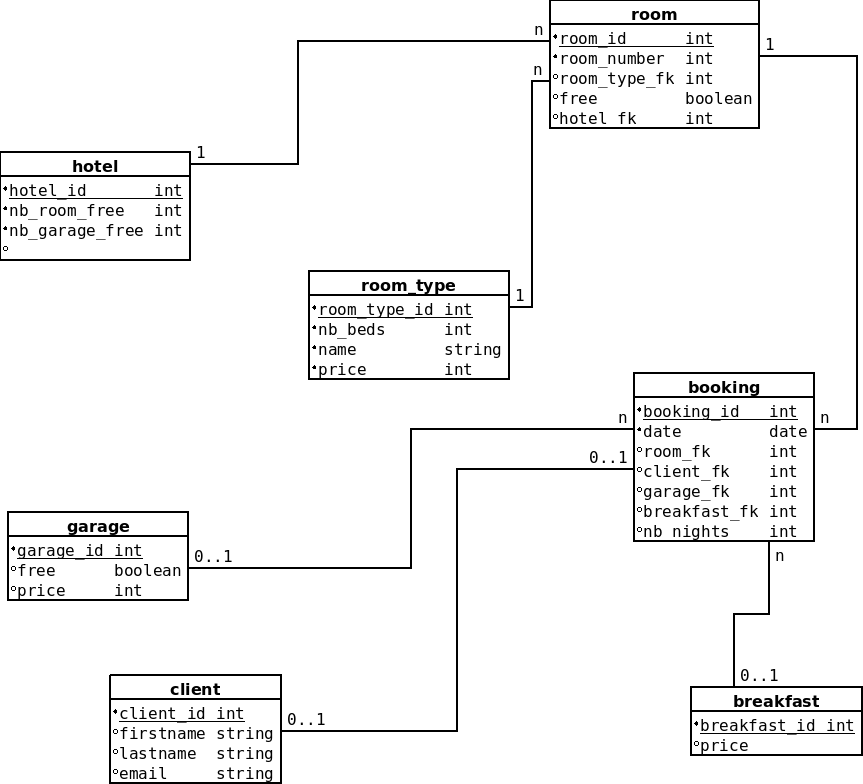
\includegraphics[height=8cm]{db.png}
\hfill \\ \\ \\
\begin{flushleft}
Le pricipe serait d'avoir toutes les informations (client, date, chambre, hotel...) via la table \textit{booking}. La table \textit{room\_type} permet d'avoir le type de chambre (nom (SR, S, JS, CD, CS ou autre), nombre de chambres...). Il y a aussi bien sur une table h\^{o}tel. La table \textit{booking} permet \'egalement de sp\'ecifier les diff\'erents services (petit d\'ejeuner, garage...).
\end{flushleft}
\hfill \\ \\
Le but est d'avoir la base de donn\'ees la plus modulable possible.
\pagebreak
\section{Microservices}
\subsection{Ajout de donn\'ees}
Ce service permettrait de pouvoir \'ecrire dans la base de donn\'ees.

\subsection{R\'ecup\'eration de donn\'ees}
Ce service permettrait de lire dans la base de donn\'ees.

\subsection{Backup}
Ce service permettrait de copier la base de donn\'ees en cas de probl\`emes.

\subsection{Ajout de log}
Ce service permettrait de pouvoir \'ecrire des logs.

\subsection{R\'ecup\'eration de log}
Ce service permettrait de pouvoir lire les logs.

\section{Routes}
\begin{itemize}
	\item /catalog\\
	r\'ecup\`ere le catalogue des chambres
	\item /frooms\\
	r\'ecup\`ere les chambres libres
\end{itemize}

\end{document}